\section{Módulos digitales utilizando VHDL}
\subsection{Compuertas básicas}
El primer ejemplo consiste en una simple red de compuertas. La figura \ref{compuertas} muestra el circuito a describir.

\begin{figure}[h]
  \centering
    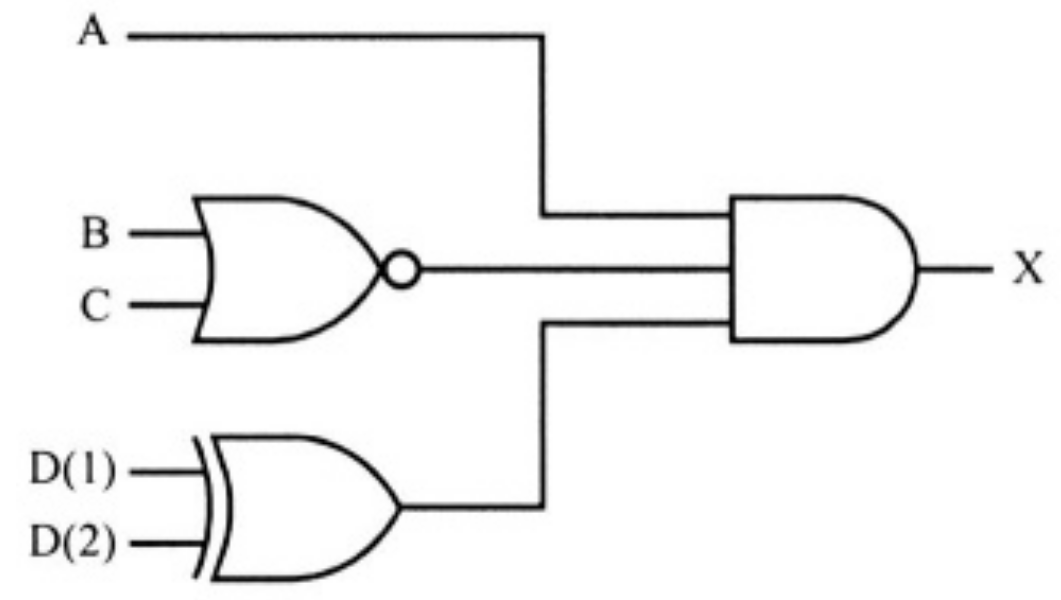
\includegraphics[width=.6\textwidth]{graficos/compuertas.png}
  \caption{Circuito digital basico basado en compuertas lógicas}
  \label{compuertas}
\end{figure}

\begin{lstlisting}[style=vhdl, basicstyle=\footnotesize\ttfamily]
--Se incluyen las librerias estandares de logica y tipos de datos
LIBRARY IEEE;
USE IEEE.STD_LOGIC_1164.ALL;

-- Normalmente el nombre de la entidad coincide con el nombre del archivo
-- Ports: Se declaran las entradas y salidas al modulo
ENTITY gate_network IS  
       PORT(A,B,C :IN STD_LOGIC;
            -- Arreglo de 2 bits
            D     :IN STD_LOGIC_VECTOR(1 DOWNTO 0);
            -- Señal de salida
            X     :OUT STD_LOGIC);
END gate_network;

-- Comienza la descripcion interna del modulo
ARCHITECTURE behavior OF gate_network IS
BEGIN                    --Sentencias concurrentes
            X <= A AND NOT( B OR C ) AND ( D( 1 ) XOR D( 2 ) );
END behavior;

            
\end{lstlisting}

\subsection{Modelo de Flip-Flops y Registros}
En el siguiente ejemplo se describirán algunas arquitecturas de flip-flops en VHDL. 
A diferencia de los dispositivos de hardware combinacionales anterior, un flip-flop sólo puede ser 
sintetizado dentro de un proceso. En VHDL ``Clock’EVENT'' es una condición verdadera siempre que 
la señal de clock cambie.

El flanco positivo se selecciona mediante `` Clock’EVENT AND clock=’1’ ''

El flanco negativo se selecciona mediante `` Clock’EVENT AND clock=’0’ ''

Para los siguientes ejemplos, la estructura del Entity y del Architecture es idéntica, sólo cambia 
el proceso interno, se definirá como puerto de salida distintos Q:

\begin{lstlisting}[style=vhdl, basicstyle=\footnotesize\ttfamily]
LIBRARY IEEE;
USE IEEE.STD_LOGIC_1164.ALL;
ENTITY DFFs IS
       PORT( D, Clock, Reset, Enable : IN STD_LOGIC;
             Q1, Q2, Q3, Q4          : OUT STD_LOGIC );
       END DFFs;
ARCHITECTURE behavior OF DFFs IS
       BEGIN 
         PROCESS
         ....
         END PROCESS;
       END behavior;
\end{lstlisting}

El flip flop de la figura \ref{ff1} es del tipo D disparado por flanco positivo
y para su implementación se utiliza WAIT para evitar el uso de listas de sensibilidad.

\begin{figure}[h!]
  \centering
    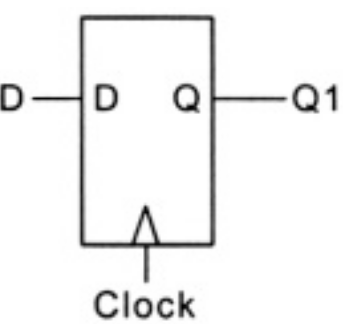
\includegraphics[width=.3\textwidth]{graficos/ff1.png}
  \caption{FF tipo D disparo por flanco positivo}
  \label{ff1}
\end{figure}

\begin{lstlisting}[style=vhdl, basicstyle=\footnotesize\ttfamily]
PROCESS
BEGIN
     WAIT UNTIL ( Clock 'EVENT AND Clock = '1');
           Q1 <= D;
END PROCESS;

\end{lstlisting}


El flip flop de la figura \ref{ff2} es del tipo D disparado por flanco positivo
con reset sincrónico.
\begin{figure}[h!]
  \centering
    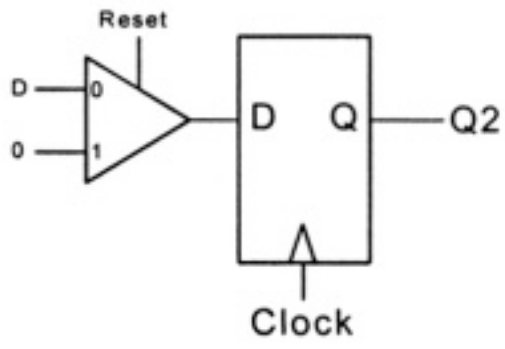
\includegraphics[width=.4\textwidth]{graficos/ff2.png}
  \caption{FF tipo D disparo por flanco positivo con reset sincrónico}
  \label{ff2}
\end{figure}

\begin{lstlisting}[style=vhdl, basicstyle=\footnotesize\ttfamily]
PROCESS
BEGIN
     WAIT UNTIL ( Clock 'EVENT AND Clock = '1');
           IF reset = '1' THEN
                Q2 <= '0';
           ELSE
                Q2 <= D;
           END IF;
END PROCESS;

\end{lstlisting}

El flip flop de la figura \ref{ff3} es del tipo D disparado por flanco positivo
con reset asincrónico. Para éste caso se utiliza la lista de sensibilidad para las
señales Reset y Clock.


\begin{figure}[h]
  \centering
    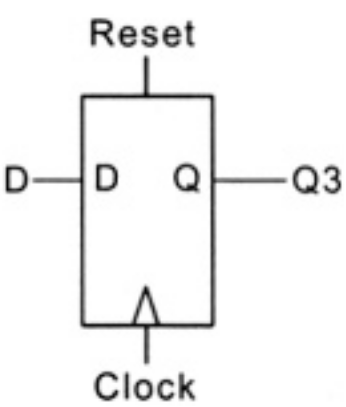
\includegraphics[width=.3\textwidth]{graficos/ff3.png}
  \caption{FF tipo D disparo por flanco positivo con reset asincrónico}
  \label{ff3}
\end{figure}


\begin{lstlisting}[style=vhdl, basicstyle=\footnotesize\ttfamily]
PROCESS (Reset,Clock)
BEGIN
     IF reset = '1' THEN
        Q3 <= '0';
     ELSIF ( clock 'EVENT AND clock = '1' ) THEN
        Q3 <= D;
     END IF;
END PROCESS;
\end{lstlisting}


El flip flop de la figura \ref{ff4} es del tipo D disparado por flanco positivo
con reset asincrónico y señal de habilitación.

\begin{figure}[h]
  \centering
    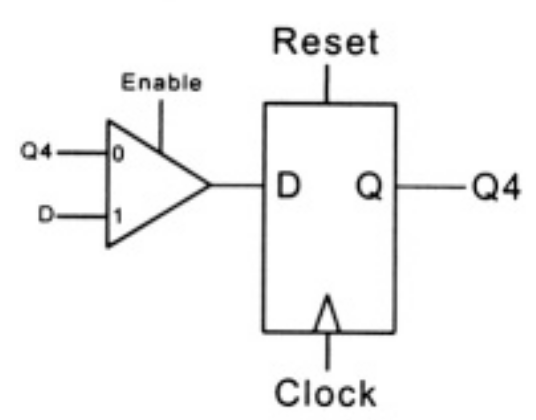
\includegraphics[width=.4\textwidth]{graficos/ff4.png}
  \caption{FF tipo D disparo por flanco positivo con reset asincrónico y habilitación}
  \label{ff4}
\end{figure}

\begin{lstlisting}[style=vhdl, basicstyle=\footnotesize\ttfamily]
PROCESS (Reset,Clock)
BEGIN
     IF reset = '1' THEN
        Q4 <= '0';
     ELSIF ( clock 'EVENT AND clock = '1' ) THEN
        IF Enable = '1' THEN
           Q4 <= D;
        END IF;
     EDN IF;
END PROCESS;
\end{lstlisting}

\subsection{Maquinas de estado sintetizadas en VHDL}
Una herramienta muy importante a la hora de trabajar en VHDL son las máquinas de estado. 
Cuando uno trabaja con circuitos digitales no hay que perder de vista que todos los procesos
que se ejecutan se realizan al mismo tiempo de forma concurrente (salvo dentro de los ``process``). 
La máquina de estados será una herramienta útil cuando se quiera realizar procesos secuenciales de forma ordenada.

En el siguiente ejemplo se describirá la máquina de Moore con tres estados, dos entradas y una salida.
El diagrama de dicha máquina se describe en la figura \ref{moore} 

\begin{figure}[h]
  \centering
    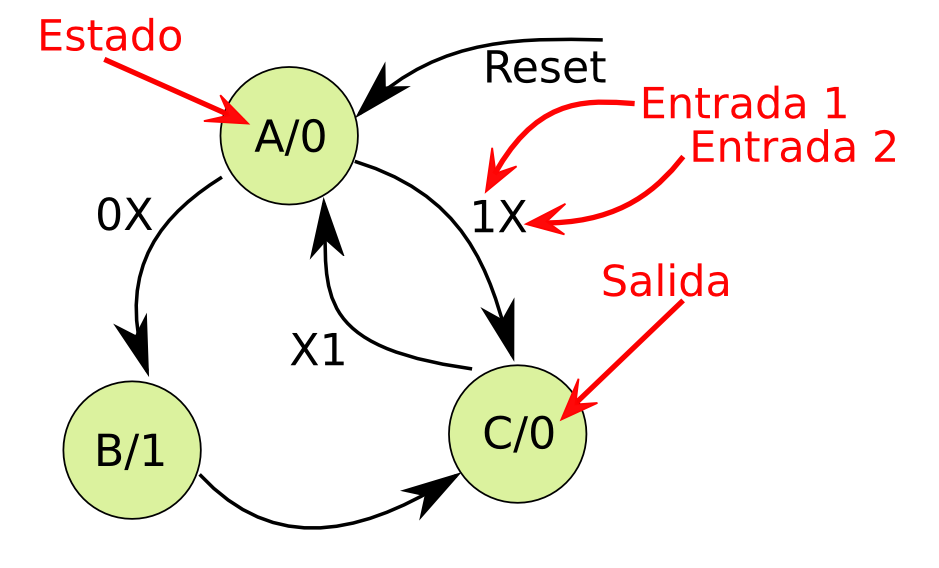
\includegraphics[width=.6\textwidth]{graficos/moore3.png}
  \caption{Máquina de estados de Moore}
  \label{moore}
\end{figure}

En VHDL, un tipo de datos enumerado se especifica, para el estado actual, con la instrucción ``TYPE''. 
Esto permite a la herramienta de síntesis asignar el valor de estado ``0'' o ``1''

Para evitar posibles problemas de ``timing``, señales externas de la maquina de estados desincronizadas, se deben
sincronizar pasando las señales a travez de flip-flops del tipo D, sincronizados con los relojes de la
máquina de estados.

\begin{lstlisting}[style=vhdl, basicstyle=\footnotesize\ttfamily]
LIBRARY IEEE;
USE IEEE.STD_LOGIC_1164.ALL;

ENTITY st_mach IS
   PORT( clk, reset      :IN STD_LOGIC;
         Input1, lnput2  :IN STD_LOGIC;
         Output1         :OUT STD_LOGIC);
END st_mach;

ARCHITECTURE A OF st_mach IS
--Enumerated Data Type for State
   TYPE STATE_TYPE IS ( state_A, state_B, state_C );
   SIGNAL state: STATE_TYPE;
BEGIN
   PROCESS ( reset, clk )
   BEGIN
      IF reset = '1' THEN   --Reset State
         state <= state_A;
      ELSIF clk 'EVENT AND clk = '1' THEN
         CASE state IS
            WHEN state_A =>
               IF Input1 = '0' THEN
                  state <= state_B;
               ELSE
                  state <= state_C;
               END IF;

            WHEN state_B =>
                  state <= state_C;

            WHEN state_C =>
               IF Input2 = '1' THEN
                  state <= state_A;
               END IF;

            WHEN OTHERS =>
                  state <= state_A;
         END CASE;
      END IF;
   END PROCESS;
   
   WITH state SELECT
      Output1 <= '0' WHEN state_A,
                 '1' WHEN state_B,
                 '0' WHEN state_C;
END A;
\end{lstlisting}

\subsection{Registro de 8 bits}
Uno de los elementos principales de todo procesador son los registros, el siguiente código 
en VHDL describe como realizar un registro de 8 bits.
port
\begin{lstlisting}[style=vhdl, basicstyle=\footnotesize\ttfamily]
LIBRARY IEEE;
USE IEEE.STD_LOGIC_1164.ALL;

ENTITY registro_8 IS
   PORT (clk, reset : in bit; 
         A          : in bit_vector(7 downto 0);
         B          : out bit_vector(7 downto 0));
   END registro_8;

ARCHITECTURE arch_reg OF registro_8 IS
BEGIN
   PROCESS(clk, reset)
   BEGIN
      IF reset=‘1’ THEN B<="00000000";
      ELSIF (clk'event and clk='1') THEN B<=A;
      END if;
   END PROCESS;
END arch_reg;
 
\end{lstlisting}

\subsection{Modelo de una ALU}
Hasta ahora hemos visto diversas estructuras y módulos simples en VHDL. Es hora de describir como 
implementar el elemento principal de todo microprocesador, la Unidad Aritmético Lógica. Para ello
realizaremos una ALU muy sencilla, que tome como entrada dos datos de 8 bits y mediante tres líneas
de control (Op\_codes) realice SUMA, RESTA, operaciones lógica AND, OR y adicionalmente le agregaremos
la opción de realizar corrimientos de datos a la salida mediante un registro de desplazamiento.
La figura \ref{alu} describe como será la estructura del código que implementaremos.
Las operaciones de los ``Op\_Codes'' se describen en la tabla \ref{aluopcodes}

\begin{figure}[h]
  \centering
    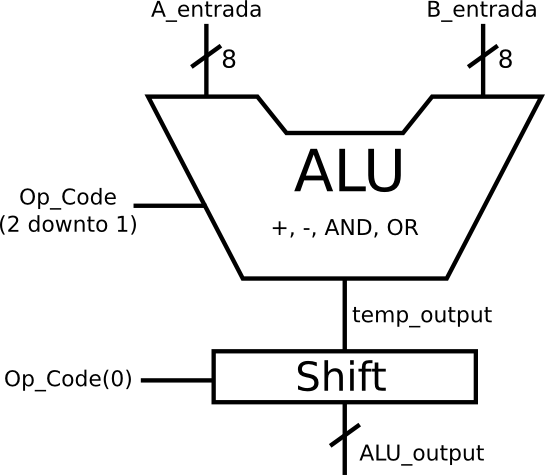
\includegraphics[width=.5\textwidth]{graficos/alu.png}
  \caption{ALU con Sumador/Restador y Desplazador}
  \label{alu}
\end{figure}

\begin{lstlisting}[style=vhdl, basicstyle=\footnotesize\ttfamily]
LIBRARY IEEE;
USE IEEE.STD_LOGIC_1164.ALL;
USE IEEE.STD_LOGIC_ARITH.ALL;
USE IEEE.STD_LOGIC_UNSIGNED.ALL;
ENTITY ALU IS
  PORT( Op_code              : IN STD_LOGIC_VECTOR( 2 DOWNTO 0 );
        A_entrada, B_entrada : IN STD_LOGIC_VECTOR( 7 DOWNTO 0 );
        ALU_output           : OUT STD_LOGIC_VECTOR( 7 DOWNTO 0 ) );
  END ALU;
ARCHITECTURE behavior OF ALU IS
   --Se describe lineas interna
   SIGNAL temp_output :STD_LOGIC_VECTOR( 7 DOWNTO 0 );
BEGIN
   PROCESS(Op_code, A_entrada, B_entrada)
   BEGIN
     CASE Op_code (2 downto 1) IS 
       WHEN "00"=>
        temp_output <= A_entrada + B_entrada;
       WHEN "01"=>
        temp_output <= A_entrada - B_entrada;
       WHEN "10"=>
        temp_output <= A_entrada AND B_entrada;
       WHEN "11"=>
        temp_output <= A_entrada OR B_entrada;
       WHEN OTHERS =>
        temp_output <= "00000000";
     END CASE

     --Operacion de desplazamiento (SHIFT)
     IF Op_code(0)='1' THEN 
       ALU_output <= temp_output(6 DOWNTO 0) & '0';
     ELSE 
       ALU_output <= temp_output;
     END_IF;
   END PROCESS;
END behavior;
\end{lstlisting}
\begin{table}[!hbt] 
\centering
 \begin{tabular}{|c|c|}
\hline
\textbf{Op\_Codes} & \textbf{Descripción} \\ \hline
000 & Suma \\ \hline
001 & Resta \\ \hline
010 & And \\ \hline
011 & Or \\ \hline
1XX & Desplazamiento \\ \hline
\end{tabular}
  \caption{Op\_codes del módulo ALU}
  \label{aluopcodes}
\end{table}  

\subsection{Modelo de una Memoria Simple}
Para explicar como se realiza una memoria realizaremos una memoria simple, con un
bus de 8 bits de datos, capacidad de 8 bytes por lo se podrá resolver con 3 bits de direccionamiento.
Para ello recurriremos a arreglos de ``standard logic vectors''. 
Esta aproximación es fácil de realizar en VHDL dado que el índice del arreglo genera 
la dirección. 
La figura \ref{ram} describe los puertos de conexión externa de la memoria

\begin{figure}[h]
  \centering
    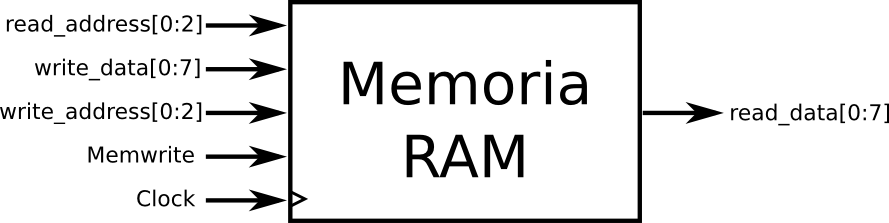
\includegraphics[width=.7\textwidth]{graficos/ram.png}
  \caption{Memoria RAM de 8 bits, capacidad 8 bytes}
  \label{ram}
\end{figure}
\begin{lstlisting}[style=vhdl, basicstyle=\footnotesize\ttfamily]
LIBRARY IEEE;
USE IEEE.STD_LOGIC_1164.ALL;
USE IEEE.STD_LOGIC_ARITH.ALL;
USE IEEE.STD_LOGIC_UNSIGNED.ALL;
ENTITY memory IS
  PORT( read_data     : OUT STD_LOGIC_VECTOR( 7 DOWNTO 0 );
        read_address  : IN STD_LOGIC_VECTOR( 2 DOWNTO 0 );
        write_data    : IN STD_LOGIC_VECTOR( 7 DOWNTO 0 ); 
        write_address : IN STD_LOGIC_VECTOR( 2 DOWNTO 0 );
        Memwrite      : IN STD_LOGIC;
        Clock         : IN STD_LOGIC );
  END memory;

ARCHITECTURE behavior OF memory IS
  --define un nuevo tipo como un arreglo de std_logic_vector
  TYPE memory_type IS ARRAY ( 0 TO 7 ) OF STD_LOGIC_VECTOR( 7 DOWNTO 0 );
  SIGNAL memory: memory_type;
BEGIN
  -- Lee la memoria y convierte el indice 
  -- del arreglo a "integer" con CONV_INTEGER
  read_data <= memory( CONV_INTEGER( read_address( 2 DOWNTO 0 ) ) ) ;
  PROCESS       --Write Memory?
  BEGIN
    WAIT UNTIL clock 'EVENT AND clock = '1';
    IF ( memwrite = '1' ) THEN
                          --convert array index to an integer with CONV_INTEGER
      memory( CONV_INTEGER( write_address( 2 DOWNTO 0 ) ) ) <= write_data;
    END IF;
  END PROCESS;
END behavior; 
\end{lstlisting}

Modelsim detecta los arreglos como memoria y permite cargar o extraer datos
para realizar la simulación. Para ello, luego de que se compila el proyecto,
en la pestaña sim, se debe seleccionar la memoria, como se indica en la figura \ref{msmemsim}

\begin{figure}[h]
  \centering
    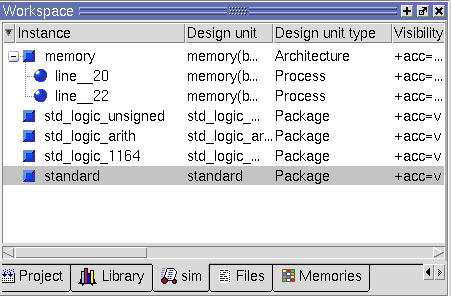
\includegraphics[width=.7\textwidth]{graficos/ms_mem1.png}
  \caption{Memoria compilada en Modelsim}
  \label{msmemsim}
\end{figure}

Luego, en la pestaña ``Memories'' se verá el arreglo (figura \ref{mem2})

\begin{figure}[h]
  \centering
    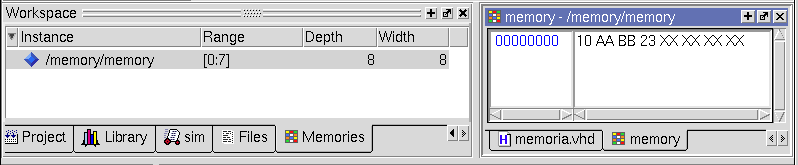
\includegraphics[width=1\textwidth]{graficos/ms_mem2.png}
  \caption{Carga y lectura de memoria en Modelsim}
  \label{mem2}
\end{figure}

Para importar o exportar datos a la memoria se utilizarán los archivos ``*.mem'' que tiene la
estructura de la figura \ref{mem3}

\begin{figure}[h]
  \centering
    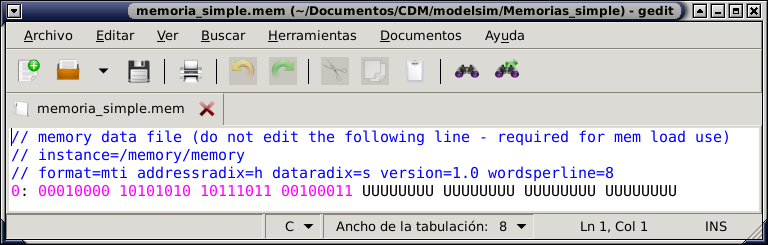
\includegraphics[width=1\textwidth]{graficos/ms_mem3.png}
  \caption{Estructura del archivo mem}
  \label{mem3}
\end{figure}

En la simulación de la figura \ref{mem4} se inicia con la memoria vacía, y se escriben los valores
``11110000'' en la dirección ``0x1'' y luego ``00001111'' en la dirección ``0x2''.

\begin{figure}[]
  \centering
    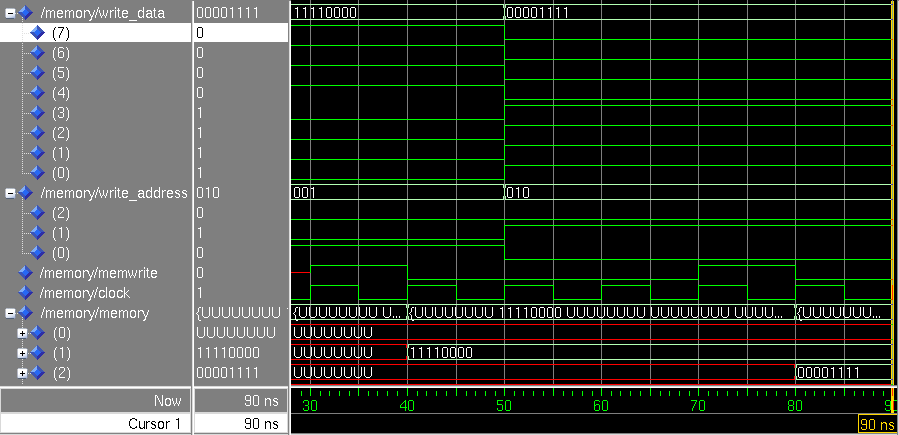
\includegraphics[width=1\textwidth]{graficos/write.png}
  \caption{Simulación del proceso de escritura}
  \label{mem4}
\end{figure}

Para simular la lectura, la memoria se inicializa con los valores de la tabla \ref{memlect}
\begin{table}[!ht] 
\centering
 \begin{tabular}{|c|c|c|c|c|c|c|c|c|}
\hline
\textbf{Dirección} & 0x0 & 0x1 & 0x2 & 0x3 & 0x4 & 0x5 & 0x6 & 0x7 \\ \hline
\textbf{Dato} & 0x00 & 0x0F & 0XF0 & 0xXX & 0xXX & 0xXX & 0xXX & 0xXX \\ \hline
\end{tabular}
  \caption{Inicialización de la memoria para simular lectura}
  \label{memlect}
\end{table}  

En la sumulación de la figura \ref{mem5} se leen las direcciones ``0x1'', ``0x2'', y ``0x0''.

\begin{figure}[]
  \centering
    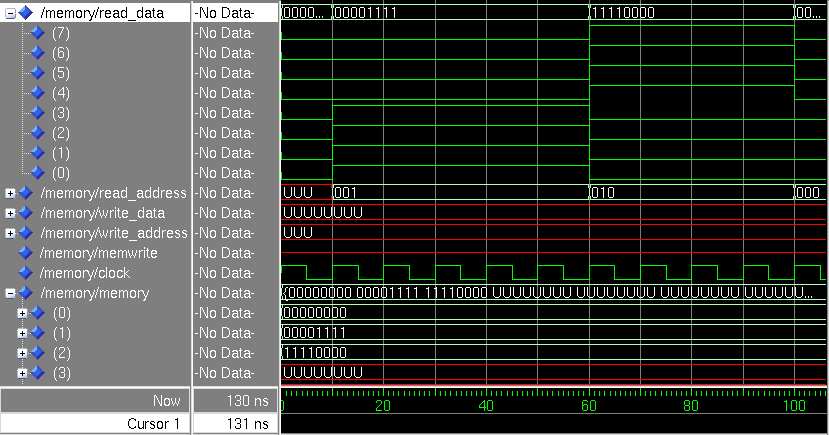
\includegraphics[width=1\textwidth]{graficos/read.png}
  \caption{Simulación del proceso de lectura}
  \label{mem5}
\end{figure}
